\documentclass[oneside]{article}
\usepackage{hyperref}
 \headheight = 25pt
\footskip = 20pt
\usepackage{graphicx}

\usepackage{mdwlist}
\usepackage[T1]{fontenc}
\renewcommand{\rmdefault}{ppl}
\usepackage{fancyhdr}
 \pagestyle{fancy}
 \lhead{\textbf{\textsc{\small Scott O'Connor\\Metaphysics}}}
 \chead{}
 \rhead{\large\textbf{\textsc{Space 2}}}
 \lfoot{\footnotesize{\thepage}}
 \cfoot{}
 \rfoot{}
 \usepackage{longtable,booktabs}
\tolerance=700


\begin{document}
\thispagestyle{fancy}



\subsection*{Introduction}

Recall Kant's argument strategy: there are spatial differences between right and left hands. But what is it about my left hand that makes it a
left hand as opposed to a right hand? There were three candidates for explaining handedness; a right hand is right because of its internal relations, or because of its relationship to other physical objects, or because of its relationships to space itself. Kant argues against the first two options, and so concludes that the final option must be the correct one; absolute space must exist to explain handedness. Thus, he concludes that Absolutism is true. 

However, the existence of higher spatial dimensions may undermine Kant's argument. Our goal in this handout is to first understand what higher spatial dimensions are meant to be. We are primarily interested in how objects could move in such dimensions. We will see that movement in a fourth dimension means that a left hand could be turned into a right hand without changing its shape---freaky! We will also see that such a possibility undermines Kant's argument against Externalism.

\subsection*{A Fourth Dimension}

The concept of higher spatial dimensions may seem peculiar. The space that we experience seems to be three dimensional. The physical objects that we experience have \emph{length}, \emph{width}, and \emph{depth}. It is difficult to conceive an object which is not so extended. Try, for instance, to conceive of a two dimensional object. That also seems impossible. But why is it impossible? Is it because there really are no two or four dimensional objects? Or is it because we are limited by the type of creatures we are? 

In the novel \emph{Flatland}, we meet creatures who live in a two dimensional space, but who are completely unable to fathom that there is a third dimension. They can move in only two dimensions, e.g., they can move left and right, backward and forward. But the idea that an object could move up or down is completely alien to them. It would be like the object disappeared in one location and reappeared in a new location. But their inability to conceive of a third dimension--and moving in a third dimension--does not entail that there is no such dimension. Their inability is just that, an inability. 

Likewise, we cannot easily imagine a fourth spatial dimension. Neither can we imagine an object moving in a fourth dimension. We conceive of objects moving upwards or downward, backwards or forwards, left or right. These seem the only option. If a fourth dimension exist, there would be a fourth dimension within to move. This means an object could vanish before our eyes and reappear somewhere new. But perhaps we struggle to conceive a fourth dimension because we are limited and not because there is no such thing. 

While we are unable to  visualize four dimensional objects, we can at least describe what they might be like and how they would move. Let us focus on a four dimensional cube. We will first describe its dimensions. We will do so by `building up' from a 1 dimensional figure. 

\begin{figure}[h]
  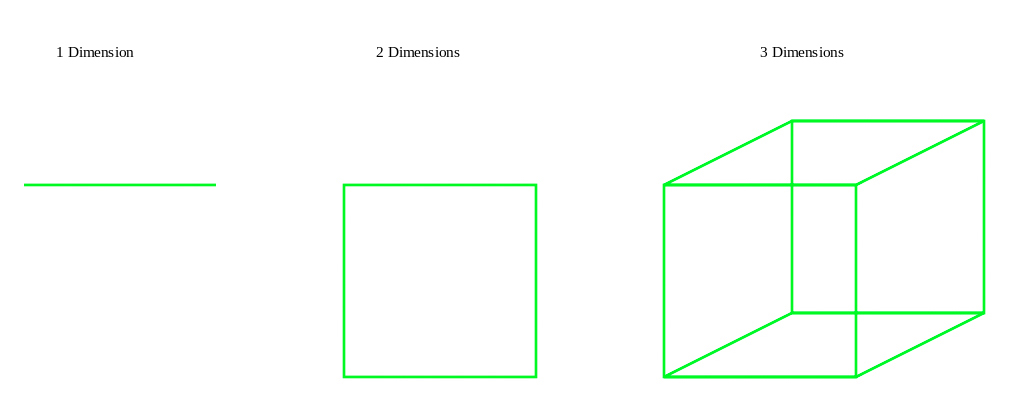
\includegraphics[width=\linewidth]{dimensions.jpg}
\end{figure}


Notice that we built up to the cube by first constructing a line; the line was extended in just one dimension. We then construct a square by moving our pencil in two dimensions, e.g., we move the pencil left to right, then down the page, then left, then upwards again. Now let us construct a cube, as depicted in the two dimensional picture on the right. We construct the cube by moving our pencil in a third dimension. If you don't quite get this, cut up some paper and construct a real cube. Once constructed, look at how the cube is extended three dimensionally. 

Just as we built up our cube from a line by allowing the pencil to move in various dimensions, a four dimensional cube could be created from the three dimensional cube if the pencil could move in a fourth dimension. One way to imagine this is by thinking of the pencil moving perpendicularly to the cube and thinking of the path of the movement as representing other parts of our four dimensional cube. If that were possible, we would create what is called a tesseract. Here is a representation of such an object. You can also find a gif on the website for this week.

\begin{figure}[h!]
\centering
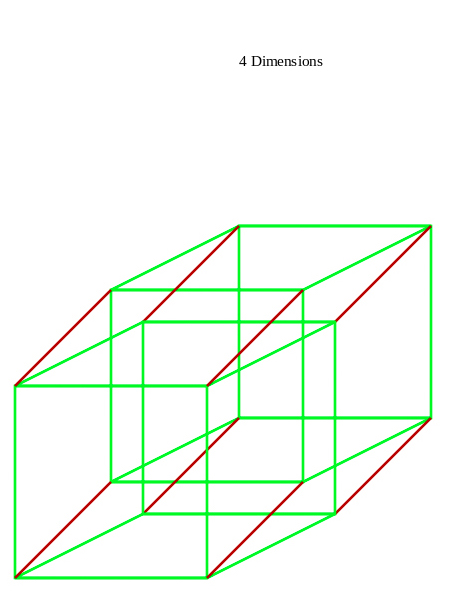
\includegraphics[width=50mm]{four.jpg}
\end{figure}

We cannot see tesseracts. But we can say things about them. A square has 4 points or vertices. A cube has 8. A tesseract has 16. Similarly, a square has 4 edges, a cube has 12, and a tesseract has 32.  Similarly, just as we can ask how many lines make up a square surface, and ask how many square surfaces make up a cube, so too we can ask how many cubes make up a tesseract. Try identify all the various cubes in the picture. (Hint: some won't look perfectly cube shape). The answer is 8! You might be surprised by this. This webpage has nice animations if you cannot count 8 by yourself: \url{http://eusebeia.dyndns.org/4d/8-cell}. How about the number of square surfaces? A tesseract has a total of 24 square surfaces. Try identify them.



\subsection*{Fourth Dimension and Incongruent Counterparts}

Recall that we defined incongruent counterparts in terms of movement: incongruent counterparts cannot be aligned via rigid movements, movements which we assumed took place in three dimensions. You cannot turn a right hand into a left hand without changing its shape or size. If higher spatial dimensions exist, then it is unclear whether there really are incongruent counterparts. For, if higher spatial dimensions exist, a right hand could be inverted and turned into a left hand, and vice versa, without changing its shape.

While this appears unusual, consider a two dimensional analogy. Suppose that you are looking down from above at a pair of triangles. Each triangle is red on one side and blue on the other. Now suppose you are asked to move the triangles to make them perfectly align. For them to perfectly align, their points must line up exactly and they must have the same color showing on each side, e.g., they must both have the blue side facing up. Now suppose you can only move the triangles in two dimensions. Can you identify the two dimensional movements that will make the triangles perfectly align in the following picture? 


\begin{figure}[h]
\centering
  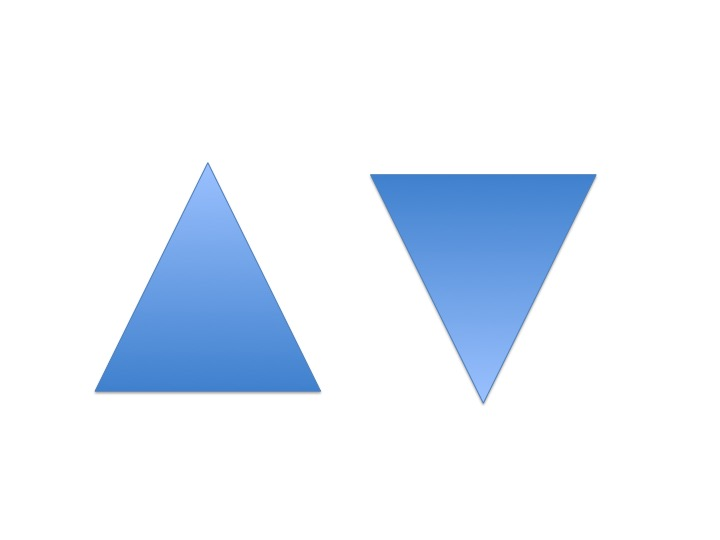
\includegraphics[width=50mm]{2d.jpg}
\end{figure}

It is easy to complete the task when our starting position is as depicted in this picture. We simply move one of the triangles backwards or forwards, left or right. How about in the following picture? (If this handout is printed in black and white, please note that left triangle has its blue surface facing upwards and the right has its red surface facing upwards.)




\begin{figure}[h]
\centering
  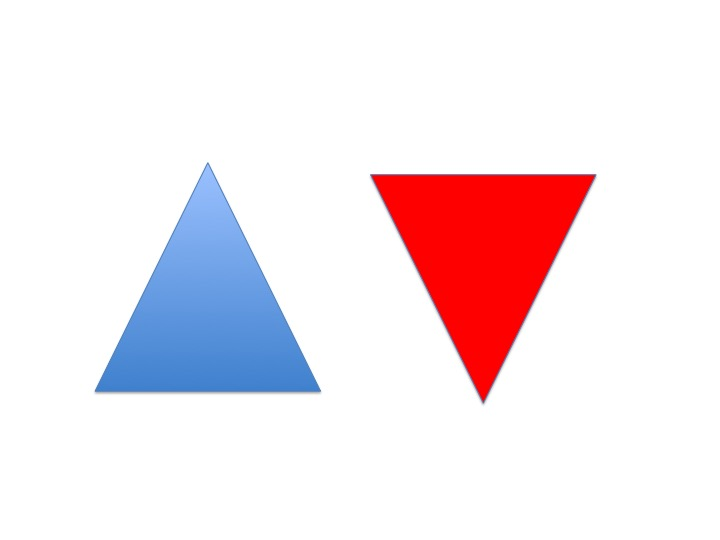
\includegraphics[width=50mm]{3d.jpg}
\end{figure}

Can you make the triangles perfectly align by only moving them in two dimensions? No! You can make their shapes align, but they will never have both their blue sides facing upwards. But once we add a third dimension, we can make both blue surfaces face upwards. We simply turn one of the triangles over.  (Cut them out if this does not make sense). When we turn a triangle over, we are moving the triangle in a third dimension, i.e., we move one point up and over the side that remains flat. 

If a creature was unable to see such a dimension, they would be unable to see such a movement.  Similarly, a creature who could not conceive of a third dimension would be unable to understand how one object could jump over or duck under another.  They could see an object ahead of them and they could see an object beside them. But they could not see an object above or below them. If, then, a kangaroo jumped over them, it would appear that the kangaroo had dematerialized in one point and rematerialized in another. Of course, the kangaroo did not do this. It just moved in a way that our two dimensional creature could not fathom. 

Likewise, if there is a fourth dimension, and if objects can move in four dimensions, then we could see the results of that motion but never actually see the motion occurring. What would the result be? Well, an object could leave a room without ever passing through a door or window. In our eyes, it would be like it dematerialized inside the room and rematerialized outside the room. We would never see the movement, but we would detect the result. Again, don't be overwhelmed by this. A two dimensional creature cannot see one thing jumping above or ducking below it. So too, we could not see an object moving in its fourth dimension. 

Recall that we could change the blue surface of the triangle from facing downwards to facing upwards by allowing a third dimension of movement. The triangle did not change shape. It was just turned over. What is the equivalent phenomenon for motion in a fourth dimension? They can be turned inside out without changing their shape! This is not equivalent to turning a glove inside out; that would result in what was inside the glove now facing outwards. I mean that we could change a right glove into a left glove, a right hand into a left hand, without changing the shape of either. See the gif on my website for an animation. This means that the hands were never incongruent counterparts; they could be made align without changing their shape through a series of movements. Just as someone might mistaking believe the triangles in the second picture are incongruent counterparts (because they are unaware of a  third dimension of movement), so too we mistakingly believe that the hands are incongruent counterparts (because we are unaware of a fourth dimension of movement.) 

 

\subsection*{Kant's Master Argument}

How does such a possibility affects Kant's argument? Recall our various options: 

\begin{description}
\item[Internalism:]  if the hands can be flipped in a fourth dimension to make them congruent, then right handedness and left handedness cannot be intrinsic properties of the  hands. In other words, Internalists say that the intrinsic features of the hands alone make  them right or left handed, but it seems a hand could be changed from left to right (and vice versa) without changing any of the intrinsic features of the hand. So, the existence of higher spatial dimensions is problematic for Internalism.
\item[Externalism:] if the hands can be flipped in a fourth dimension to make them congruent, then 
a hand does not have handedness if it exists all alone in the Universe. In other words, Kant's claim that a solitary hand must be either left or right before a body pops into existence is false. The hand can fit perfectly on either wrist by rotating it in a fourth dimension. Thus, Kant's argument against Externalism fails. 

\item[Absolutism:] Kant argued for this position by eliminating Internalism and Externalism. But since the existence of a fourth spatial dimension undermines his argument for Externalism, he cannot claim to have eliminated Externalism. Therefore, he cannot claim to have establish the existence of absolute space 
\end{description}

\noindent \emph{Score-keeping:} do higher spatial dimensions exist? We have not tried to prove their existence. Rather, we have shown that the possibility of their existence undermines Kant's argument for Absolutism. But this does not prove that Absolutism is false. If Kant can show that there are no higher spatial dimensions, then his argument for Absolutism will be secured. If a Relationalist dislikes higher spatial dimensions, then they must find some alternative way of undermining Kant's argument. 



\end{document}
